\documentclass[11pt]{article}
\usepackage{worksheet_style}

% ---- Toggle: uncomment for filled version ----
%\worksheetfilledtrue
\begin{document}
\worksheetheader{9}{Limits and Continuity in Several Variables}

\begin{background}
Before we can differentiate multivariate functions, we need limits. The key new difficulty: in one variable, you approach a point from the left or right. In two variables, you can approach from infinitely many directions. This makes proving limits exist much harder---and gives us a powerful tool (path analysis) for showing they don't.
\end{background}

%=============================================================
\wsection{Multivariable Limits}

\begin{defbox}{Limit of $f(x,y)$ as $(x,y)\to(a,b)$}
We write $\ds\lim_{(x,y)\to(a,b)} f(x,y) = L$ if $f(x,y)$ can be made arbitrarily close to $L$ for all $(x,y)$ sufficiently close to $(a,b)$.

\medskip
\textbf{Key difference from single-variable:}
\begin{itemize}[nosep]
  \item In 1D -- only \wbi{two directions}{2.5cm} (left and right)
  \item In 2D -- must approach from \wbi{infinitely many directions and paths}{5cm}
  \item If \textit{any two paths} give different limits $\implies$ limit \textbf{DNE}
\end{itemize}
\end{defbox}

\begin{formulabox}{Properties of Multivariable Limits}
If $\ds\lim_{(x,y)\to(a,b)} f = L$ and $\ds\lim_{(x,y)\to(a,b)} g = M$ exist:
\begin{multicols}{2}
\begin{itemize}[nosep, leftmargin=*]
  \item $\lim(f \pm g) = L \pm M$
  \item $\lim(cf) = cL$
  \item $\lim(fg) = LM$
  \item $\lim(f/g) = L/M$ if $M \neq 0$
\end{itemize}
\end{multicols}
Polynomials and rational functions (where defined) -- use \textbf{direct substitution}.
\end{formulabox}

%=============================================================
\wsection{Techniques for Evaluating Limits}

\wsubsection{Technique 1: Direct Substitution}

-- Always try first; works when $f$ is continuous at $(a,b)$

\wsubsection{Technique 2: Algebraic Simplification / Rationalization}

-- Factor, multiply by conjugate, or simplify before substituting

\begin{example}[Rationalization]
Evaluate $\ds\lim_{(x,y)\to(1,1)} \frac{\sqrt{x} - \sqrt{y}}{x - y}$.

\wbbox{
\textbf{1. Rationalize:}

$\frac{\sqrt{x}-\sqrt{y}}{x-y} \cdot \frac{\sqrt{x}+\sqrt{y}}{\sqrt{x}+\sqrt{y}} = \frac{x-y}{(x-y)(\sqrt{x}+\sqrt{y})} = \frac{1}{\sqrt{x}+\sqrt{y}}$

\textbf{2. Substitute:}

$\ds\lim_{(x,y)\to(1,1)} \frac{1}{\sqrt{x}+\sqrt{y}} = \frac{1}{1+1} = \boxed{\frac{1}{2}}$
}{3.5cm}
\end{example}

\wsubsection{Technique 3: Polar / Spherical Coordinates}

-- For limits at the origin: $x = r\cos\theta$, $y = r\sin\theta$, $(x,y)\to(0,0) \iff r\to 0^+$

-- If the result is independent of $\theta$ and tends to $L$ as $r\to 0$, the limit is $L$

\begin{example}[Polar Coordinates]
Evaluate $\ds\lim_{(x,y,z)\to(0,0,0)} \frac{\sin(x^2+y^2+z^2)}{x^2+y^2+z^2}$.

\wbbox{
\textbf{1. Convert:} In spherical coordinates, $x^2+y^2+z^2 = \rho^2$

\textbf{2. Simplify:} $\ds\lim_{\rho\to 0^+} \frac{\sin(\rho^2)}{\rho^2}$

\textbf{3. Evaluate:} Let $u = \rho^2 \to 0$: $\ds\lim_{u\to 0}\frac{\sin u}{u} = \boxed{1}$
}{3cm}
\end{example}

\wsubsection{Technique 4: Path Analysis (for showing DNE)}

-- If two different paths give different limiting values $\implies$ limit DNE

\begin{formulabox}{Common Paths to Try}
\begin{itemize}[nosep, leftmargin=*]
  \item Along axes: $y = 0$, then $x = 0$
  \item Along lines: $y = mx$ for various $m$
  \item Along curves: $y = x^2$, $y = x^3$, etc.
\end{itemize}
If all linear paths give the same value -- try a curved path before concluding the limit exists!
\end{formulabox}

\begin{center}
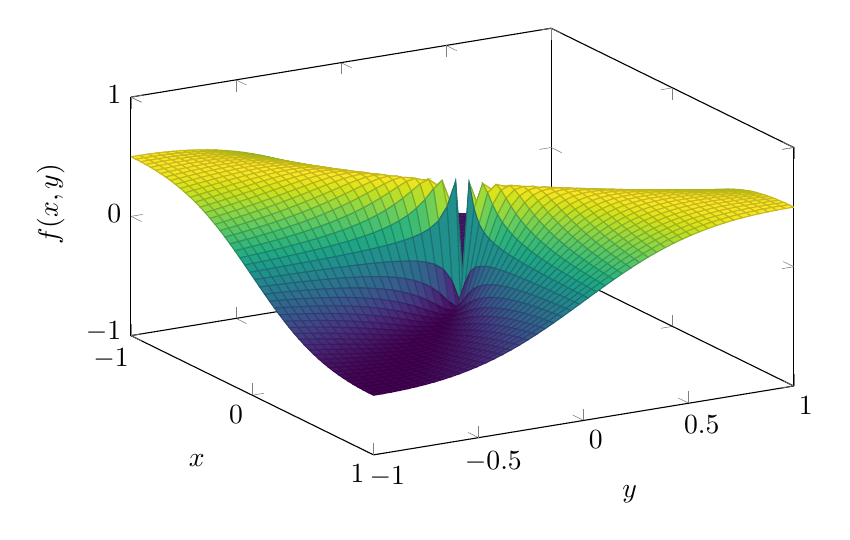
\begin{tikzpicture}
\begin{axis}[
    view={60}{30},
    xlabel={$x$},
    ylabel={$y$},
    zlabel={$f(x, y)$},
    domain=-1:1,
    y domain=-1:1,
    samples=50,
    samples y=50,
    zmin=-1,
    zmax=1,
    colormap/viridis,
    width=10cm, height=7cm,
]
\addplot3[surf] {x*y/(x^2 + y^2)};
\end{axis}
\end{tikzpicture}\\
{\small Graph of $z = \dfrac{xy}{x^2+y^2}$ near the origin. The surface takes different limiting values along different paths to $(0,0)$: along $y=0$ or $x=0$ it equals $0$, but along $y=x$ it equals $1/2$. Hence the limit does not exist.}
\end{center}

\begin{example}[Limit DNE by Path Analysis]
Show $\ds\lim_{(x,y)\to(0,0)} \frac{x^2 - y^2}{x^2 + y^2}$ does not exist.

\wbbox{
\textbf{1. Path along $y = 0$:} $\frac{x^2-0}{x^2+0} = 1 \implies$ limit $= 1$

\textbf{2. Path along $x = 0$:} $\frac{0-y^2}{0+y^2} = -1 \implies$ limit $= -1$

\textbf{3. Result:} $1 \neq -1$, so the limit \textbf{DNE}.
}{3cm}
\end{example}

\begin{example}[Tricky: All Lines Give 0, But Limit DNE]
Does $\ds\lim_{(x,y)\to(0,0)} \frac{xy^2}{x^2 + y^4}$ exist?

\wbbox{
\textbf{1. Along $y = mx$:} $\frac{x \cdot m^2 x^2}{x^2 + m^4 x^4} = \frac{m^2 x}{1+m^4 x^2} \to 0$ as $x\to 0$

Every straight line gives limit $= 0$.

\textbf{2. Along $x = y^2$:} $\frac{y^2 \cdot y^2}{y^4 + y^4} = \frac{y^4}{2y^4} = \frac{1}{2}$

\textbf{3. Result:} $0 \neq 1/2$, so the limit \textbf{DNE}.

\textit{Lesson:} Checking only straight-line paths is not sufficient!
}{4.5cm}
\end{example}

%=============================================================
\wsection{Continuity}

\begin{defbox}{Continuity of $f(x,y)$}
$f$ is \textbf{continuous at $(a,b)$} if all three hold:
\begin{enumerate}[nosep]
  \item $f(a,b)$ is defined
  \item $\ds\lim_{(x,y)\to(a,b)} f(x,y)$ exists
  \item $\ds\lim_{(x,y)\to(a,b)} f(x,y) = f(a,b)$
\end{enumerate}

\wb{Polynomials, exponentials, trig functions, and their compositions are continuous on their domains.}
\end{defbox}

%=============================================================
\begin{practice}

\prob
Evaluate $\ds\lim_{(x,y)\to(2,3)} (x^2 y + xy^2 - 1)$.

\wans{\wbml{$(4)(3) + (2)(9) - 1 = 12+18-1 = 29$}}

\vspace{2cm}

\prob
Evaluate $\ds\lim_{(x,y)\to(0,0)} \frac{x^2 y}{x^2 + y^2}$.

\wbbox{
Polar: $\frac{r^2\cos^2\theta \cdot r\sin\theta}{r^2} = r\cos^2\theta\sin\theta$

$|r\cos^2\theta\sin\theta| \leq r \to 0$, so the limit is $\boxed{0}$ by Squeeze Theorem.
}{3cm}

\prob
Show $\ds\lim_{(x,y)\to(0,0)} \frac{xy}{x^2 + y^2}$ does not exist.

\wbbox{
Along $y=0$: $0/x^2 = 0$, limit $= 0$.

Along $y=x$: $x^2/(2x^2) = 1/2$, limit $= 1/2$.

$0 \neq 1/2 \implies$ DNE.
}{3cm}

\prob
Evaluate $\ds\lim_{(x,y)\to(1,1)} \frac{x^2 - y^2}{x - y}$.

\wbbox{
Factor: $\frac{(x-y)(x+y)}{x-y} = x+y \to 1+1 = \boxed{2}$ \; (cancel since $x\neq y$ in the limit).
}{2cm}

\prob
Show $\ds\lim_{(x,y)\to(0,0)} \frac{x^2 y^2}{x^2 y^2 + (x-y)^2}$ does not exist.

\wbbox{
Along $y=0$: $\frac{0}{0+x^2} = 0$, limit $= 0$.

Along $y=x$: $\frac{x^4}{x^4+0} = 1$, limit $= 1$.

$0 \neq 1 \implies$ DNE.
}{3cm}

\prob
Prove using $\epsilon$-$\delta$ that $\ds\lim_{(x,y)\to(0,0)} \frac{3x^2 y}{x^2+y^2} = 0$.

\textit{Hint:} Use $|y| \leq \sqrt{x^2+y^2}$.

\wbbox{
$\left|\frac{3x^2 y}{x^2+y^2}\right| = 3\cdot\frac{x^2}{x^2+y^2}\cdot|y| \leq 3 \cdot 1 \cdot |y| \leq 3\sqrt{x^2+y^2}$

Given $\epsilon > 0$, choose $\delta = \epsilon/3$. If $\sqrt{x^2+y^2} < \delta$:

$\left|\frac{3x^2 y}{x^2+y^2}\right| \leq 3\sqrt{x^2+y^2} < 3\delta = \epsilon$. \quad $\square$
}{4cm}

\end{practice}

\end{document}
